\documentclass[10pt]{article}
\usepackage{/home/liam/4thlabs/latex/lab}


\title{Assignment 1 - Advanced Computational Science}

\newcommand{\ujn}{u_{j}^{n}}
\newcommand{\ujpn}{u_{j+1}^{n}}
\newcommand{\ujmn}{u_{j-1}^{n}}
\newcommand{\ujnp}{u_{j}^{n+1}}
\newcommand{\ujnm}{u_{j}^{n-1}}
\newcommand{\eihjk}{e^{ikhj}}
\newcommand{\eihjpk}{e^{ikh(j+1)}}
\newcommand{\eihjmk}{e^{ikh(j-1)}}

\begin{document}
\maketitle

\section*{Question 1}
\subsection*{(1)}
We are interested in solving the 1-d wave equation with $c=1$,
\begin{equation}
\frac{\partial^2 u}{\partial t^2} = \frac{\partial^2 u}{\partial x^2}
\label{e:we}
\end{equation}
using central differences,
\begin{equation}
\frac{\partial^2 u}{\partial t^2} \approx \frac{\delta_t^2 \ujn}{\tau^2},
\hspace{5mm}
\frac{\partial^2 u}{\partial x^2} \approx \frac{\delta_x^2 \ujn}{h^2}
\label{e:central}
\end{equation}
so our equation becomes
\begin{equation}
\frac{\delta_t^2 \ujn}{\tau^2} = \frac{\delta_x^2 \ujn}{h^2}
\label{e:wecd}
\end{equation}
where $\tau$ is the time step size, and $h$ is the $x$ step size.

The operator $\delta_x ^2$, when applied to $\ujn$, gives
$$
\delta_x^2 = \ujnm - 2\ujn + \ujnp
$$
allowing us to expand out for both spatial and temporal derivatives and rearrange
for $\ujnp$, giving
\begin{equation}
\ujnp = \nu^2 \left[\ujmn + \ujpn \right] - \ujnm + 2(1 - \nu^2)\ujn
\label{e:cd}
\end{equation}
with $\nu = \frac{\tau}{h}$.

A program was written in Python 3.3 to solve this problem with Dirichlet boundary
conditions, $u(-7,t) = u(7,t) = 0$, on the intervals $x \in \left[-7,7\right]$,
$t \in \left[0,14\right] $. The boundaries are imposed by only computing from
$j=1$ to $j=j_\text{max} -1$, neglecting both endpoints in the array, as the entire
array is initialised to 0.
The initial condition is given by $u(x,0) = e^{-x^2}$.
The program is included in appendix \ref{a:1.1}.
Values for $h,\tau$ were taken to be $h=0.1$ and $\tau = \frac{1}{10\sqrt{2}}$, with
$\tau$ set by $h$ as discussed in section 1.2, and $h$ justified in section 1.3.

The solutions at various times are shown in figure \ref{f:dirichlet}.
\begin{figure}
  \centering
  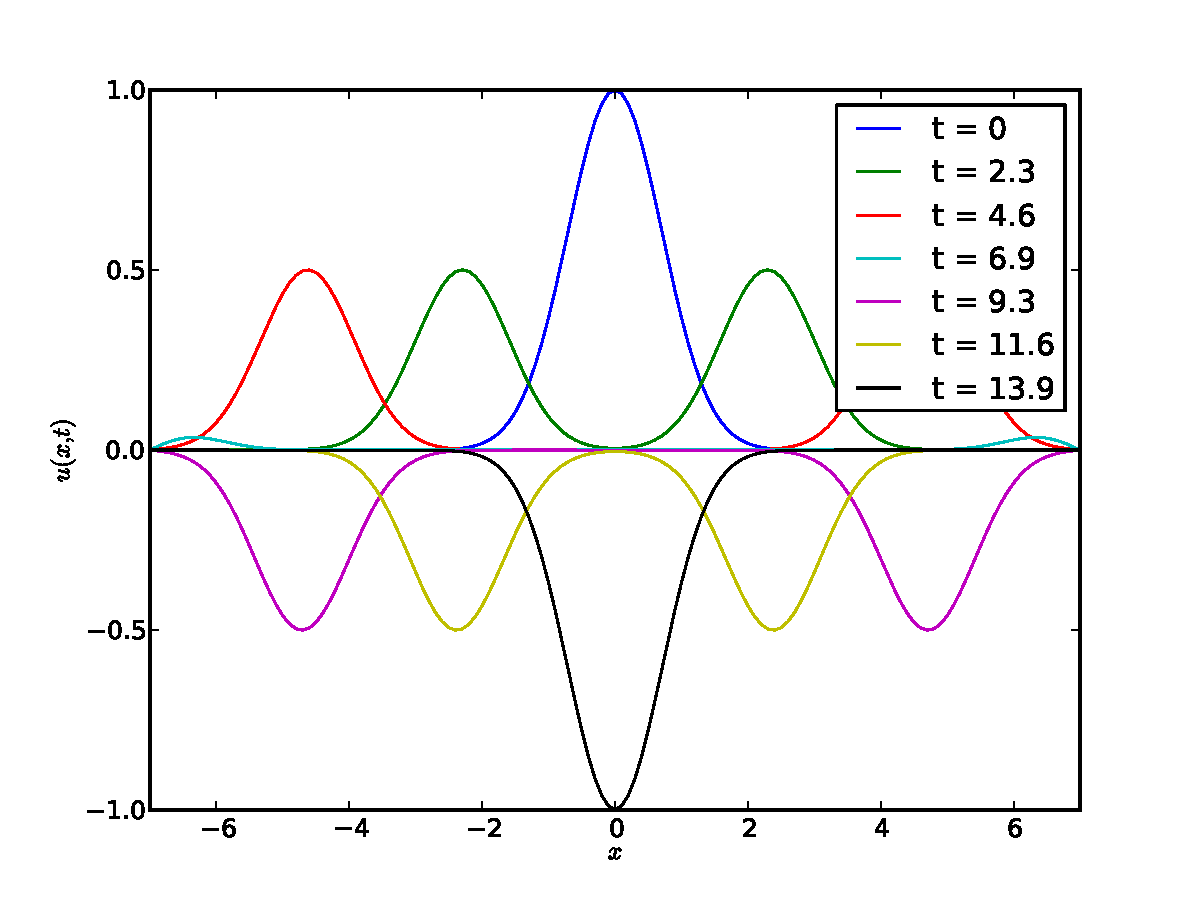
\includegraphics[width=\textwidth]{1/dirichlet.pdf}
  \caption{Solution to the wave equation with Gaussian initial condition, $h=0.1$.}
  \label{f:dirichlet}
\end{figure}
The wave is observed to split in two, propagating half in either direction.
At the boundaries, the wave is inverted, travelling back to superimpose into
a mirror image of the initial condition at $t=14$.

\clearpage
\subsection*{(2)}
Our expression for $\ujn$ using Central Differences is given in equation \ref{e:cd}.
To perform Fourier/von Neumann stability analysis, we take $\ujn = \xi^n \eihjk$ as
a single Fourier mode solution, and see how our {\it amplification factor}, $\xi$,
behaves as a function of $\tau,h,k$.
Substituting this into equation \ref{e:cd} gives
$$
\xi^{n+1} \eihjk= \nu^2 \left[ \xi^n \eihjmk + \xi^n \eihjpk \right] - \xi^{n-1} \eihjk +
2(1 - \nu^2) \xi^n \eihjk.
$$
Dividing across by $\xi^{n-1} \eihjk$ and cleaning up gives
\begin{equation}
\xi^2 + \alpha \xi + 1 = 0
\label{e:quad}
\end{equation}
with
$$\alpha = -\nu^2 \left[ e^{-ikh} + e^{ikh} - 2\left(1 - \frac{1}{\nu^2}\right) \right]
= -2 \nu^2 \left[ \cos(kh) - \left(1 - \frac{1}{\nu^2}\right) \right] $$
$$= -2 \nu^2 \left[ 1 - \sin^2\left(\frac{kh}{2}\right) - \left(1 - \frac{1}{\nu^2}\right) \right]
=  2 \nu^2 \left[ \sin^2\left(\frac{kh}{2}\right) - \frac{1}{\nu^2} \right] $$
This is a quadratic equation with roots
$$
\xi_\pm = \frac{1}{2} \left( -\alpha \pm \sqrt{\alpha^2 - 4} \right) =
\frac{1}{2} \left( -\alpha \pm i\sqrt{(2 - \alpha)(2+\alpha)}\right).
$$
Inserting $\alpha$ into the above gives
$$ \xi_\pm = -\frac{1}{2}\left[2\nu^2 \sin^2\left(\frac{kh}{2}\right) -1 \right]
\pm \frac{1}{2}\sqrt{\left(4\nu^2\sin^2\left(\frac{kh}{2}\right) -2\right)^2 - 4}
$$
$$ = -\left[2\nu^2 \sin^2\left(\frac{kh}{2}\right) -1 \right]
\pm \nu\sin\left(\frac{kh}{2}\right)\sqrt{4\nu^2\sin^2\left(\frac{kh}{2}\right) -2}
$$

We consider $\tau >0$ and $h>0$, and by extension $\nu>0$.
From here, it is immediately apparent that if $\nu >1$, both terms will be greater
than $1$ for some values of $k$, making the method unstable.
For $\nu = 1$, $|\xi_-|$ can for some values of $k$, be greater than one.
A good choice seems to be $\nu = \frac{1}{\sqrt{2}}$, as then the above reduces to
$$\xi_\pm = -\left[\sin^2\left(\frac{kh}{2}\right) - 1 \right] \pm \sin\left(\frac{kh}{2}\right)
\sqrt{\sin^2\left(\frac{kh}{2}\right) -1}$$
$$= -\left[\sin^2\left(\frac{kh}{2}\right) - 1 \right] \pm \sin\left(\frac{kh}{2}\right)
\sqrt{-\cos^2\left(\frac{kh}{2}\right)}$$
$$= -\left[\sin^2\left(\frac{kh}{2}\right) - 1 \right] \pm i\sin\left(\frac{kh}{2}\right)
\cos\left(\frac{kh}{2}\right)$$
In the limits of $h \to 0$ or $k \to 0$, the sin terms go to 0, and we are left with
$\xi_\pm = 1$. Elsewhere, the function moves between 0 and 1 as a function of $k$.
Otherwise, when considering $|\xi_\pm|$, it is calculated by
$$ \xi_\pm = \sqrt{\text{Re}\left(\xi_\pm\right)^2 + \text{Im}\left(\xi_\pm\right)^2}.$$
This demonstrates that $\xi_+$ and $\xi_-$ are equivalent for $\nu=\frac{1}{\sqrt{2}}$.
It is worth noting that in
the above workings on the expression for $\xi_\pm$, many $\pm$s were absorbed by the
initial $\pm$ due to working with the square root. This leads me to believe that both
$\xi_\pm$ are not physically significant.
In the quadratic form, we consider what happens when we require $\xi \in [-1,1]$.
It is clear that $\alpha$ as defined earlier must be bound to the region $[-2,2]$,
which sets a clear requirement that $\nu \in (0,1]$\footnote{$\nu$ could be negative, but
we have previously constrained it to be positive.}
is a limit beyond which stability will not be achieved. This constrains
$\tau \le h$ for stability.
However, I have chosen to take $\nu = \frac{1}{\sqrt{2}}$
for the computations in this report, a situation where $\xi \in [0,1]$ is guaranteed,
as this avoids the possibility of one of $\xi_\pm$ blowing the solution up, should I be wrong.

{\it Note}: $\nu = 1$ was tested in these exercises and did not lead to the solution
blowing up in the time intervals used.

\clearpage
\subsection*{(3)}
In order to find an optimal value of $h$ for our solutions, we define the {\it relative
error},
\begin{equation}
\epsilon (h) = 1 - \frac{L_{h/2}}{L_h}
\label{e:err}
\end{equation}
where $L_h$ is the $L^2$-norm of the solution computed with $h$, and $L_\frac{h}{2}$ with
$\frac{h}{2}$.
The $L^2$-norm is computed numerically as
\begin{equation}
L_h  = \sqrt{h\cdot \sum_{j=0}^{j_\text{max}} u_{j}^{t=10.5}}
\label{e:l2}
\end{equation}
at $t=10.5$.

A program was written in Python 3.3 to compute this function for various values of
$h$, available in appendix \ref{a:1.4}. The program defines a function which takes
the $h$ value as an argument, performs the integration, and then returns the $L^2$-norm
at $t=10.5$. As such, for each $h$ value, this is called twice; once for $h$ and once for
$\frac{h}{2}$.
Plotted in figure \ref{f:hstudy1} is the function $\epsilon(h)$ for various values of $h$.
We are told to choose a value of $h$ such that the relative error is $\approx 10^{-3}$.
As such, I chose $0.1$, as this is a round number giving relative error
$\epsilon \approx 3\times10^{-4}$.
\begin{figure}
  \centering
  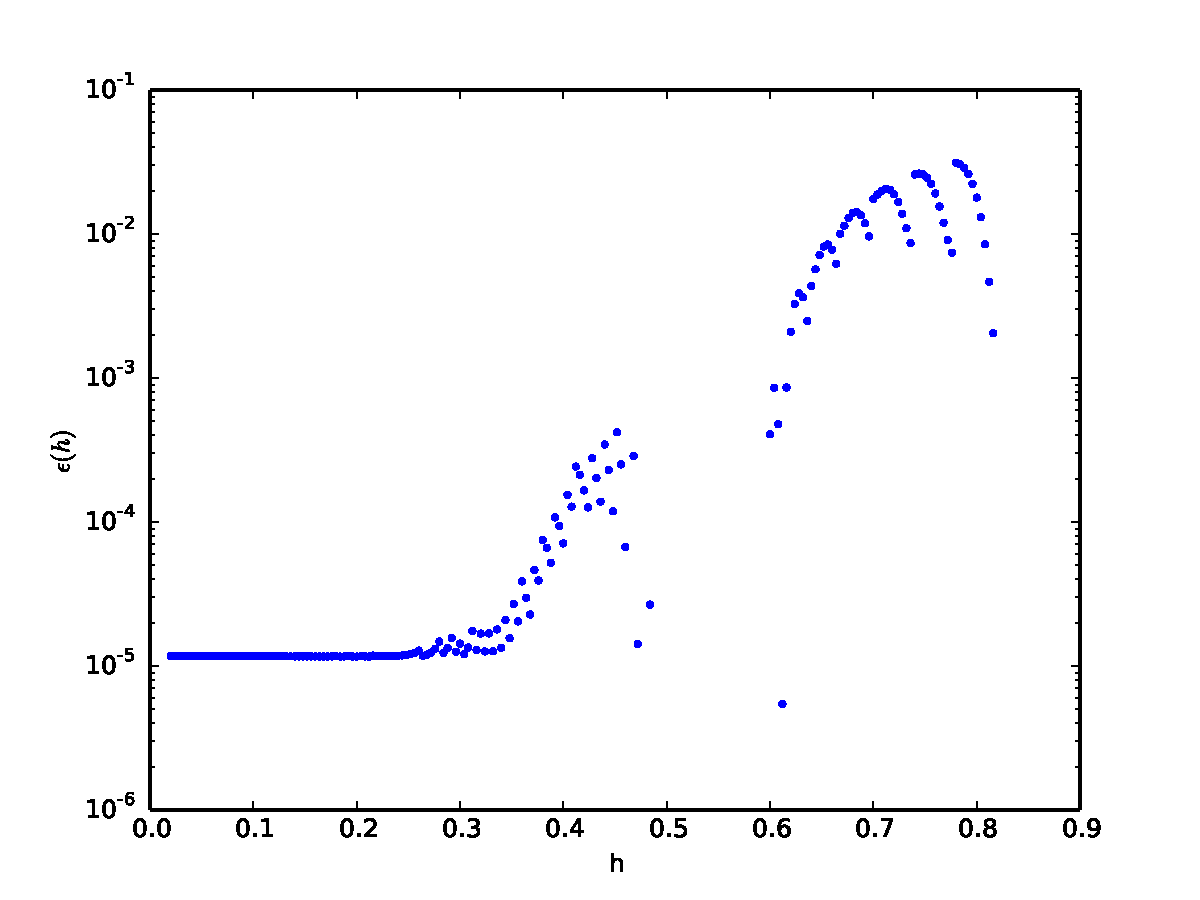
\includegraphics[width=\textwidth]{1/Error.pdf}
  \caption{Relative error as a function of $h$.}
  \label{f:hstudy1}
\end{figure}


\clearpage
\subsection*{(4)}
This exercise is a repeat of the first, but using Neumann boundary conditions;
$\frac{\partial}{\partial x}(x_\text{min}) = \frac{\partial}{\partial x}(x_\text{max})
= 0$.
These were imposed by setting $u_0 ^n = u_1^n$ and equivalent on the max boundary.
The program used is included in appendix \ref{a:1.4}.
The solutions to the problem at various times are plotted in figure \ref{f:neumann},
showing the wave initially propagate as in section 1.1, but proceeding to reflect
from the walls without inverting as before.
\begin{figure}
  \centering
  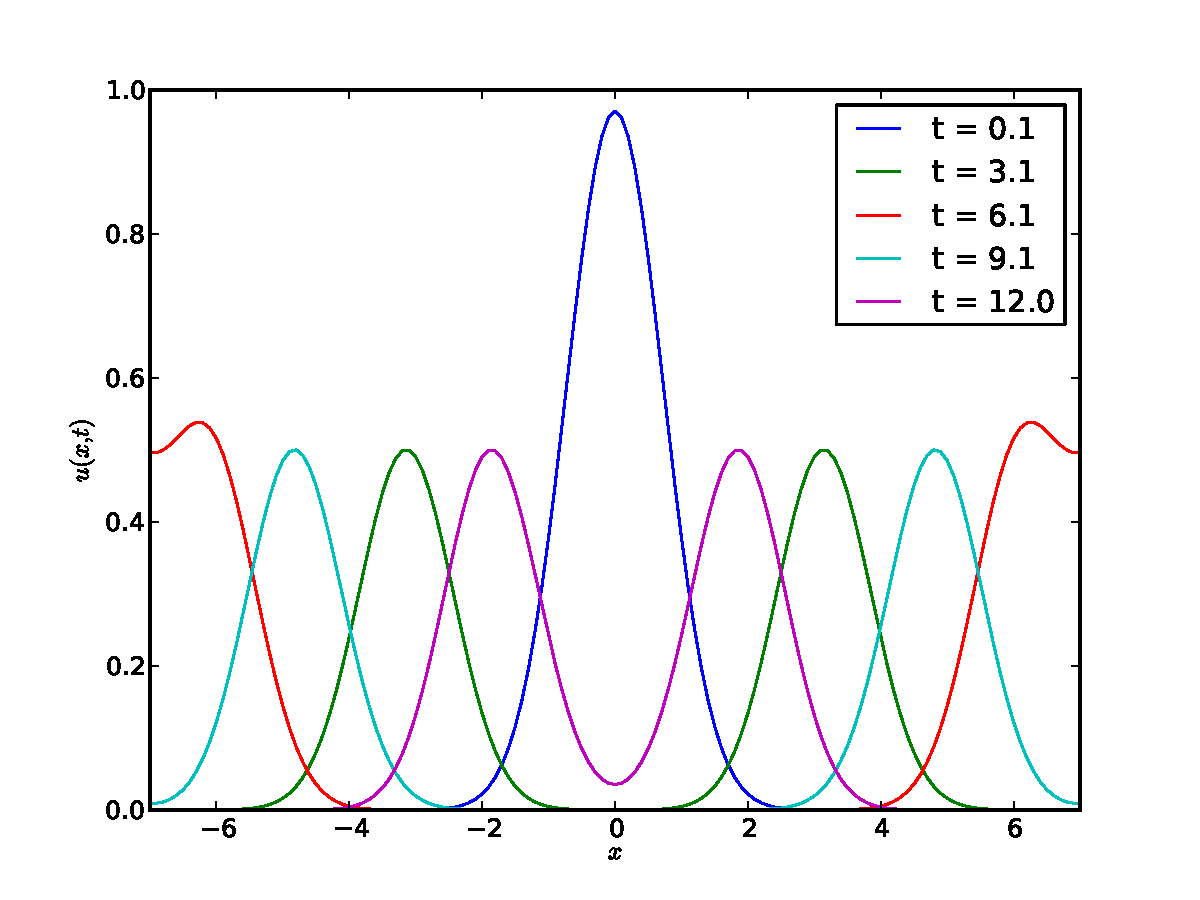
\includegraphics[width=\textwidth]{1/neumann.pdf}
  \caption{Solution to the wave equation with Gaussian initial condition
           with Neumann boundaries.}
  \label{f:neumann}
\end{figure}


\clearpage
\subsection*{(5)}
\subsubsection*{Analytical Energy Conservation}
\begin{equation}
\mathcal{H}(x,t) = \frac{1}{2}\left( \frac{\partial u}{\partial t}\right)^2
+ \frac{1}{2}\left( \frac{\partial u}{\partial x}\right)^2
\label{e:hd}
\end{equation}

\begin{equation}
E(t) = \int_{x_\text{min}}^{x_\text{max}} \mathcal{H}(x,t) dx
\label{e:energy}
\end{equation}
\subsubsection*{Numerical Results}
The Hamiltonian density is defined in equation \ref{e:hd}. As such, we compute an
array of values, $\mathcal{H}_j^n$. At the boundaries of space or time,
forward/backward differences are used in that quantity, with Double-Interval
central differences used elsewhere, for example
$$ \mathcal{H}_j^n = \frac{1}{2}\left[\frac{1}{2\tau}\left(\ujnp - \ujnm\right)\right]^2
+ \frac{1}{2}\left[ \frac{1}{2h} \left(\ujpn - \ujmn\right)\right]^2 $$
generally, with variations where $j = 0 , j_\text{max}$, etc.
As in the case for $L^2$-norms, we perform naive integration
$$E^n = h\sum_j \mathcal{H}_j^n. $$

\noindent To quantify the conservation of energy, we define the {\it relative error},
\begin{equation}
f_r (t) = \frac{E(t) - E(0)}{E(0)}.
\label{e:relerr}
\end{equation}
This is implemented in the programs presented in appendix \ref{a:1.5}, written in Python 3.3.
Figure \ref{f:relerr} shows this quantity as a function of time for the problem
posed in sections 1.1 and 1.4.

\begin{figure}
  \centering
  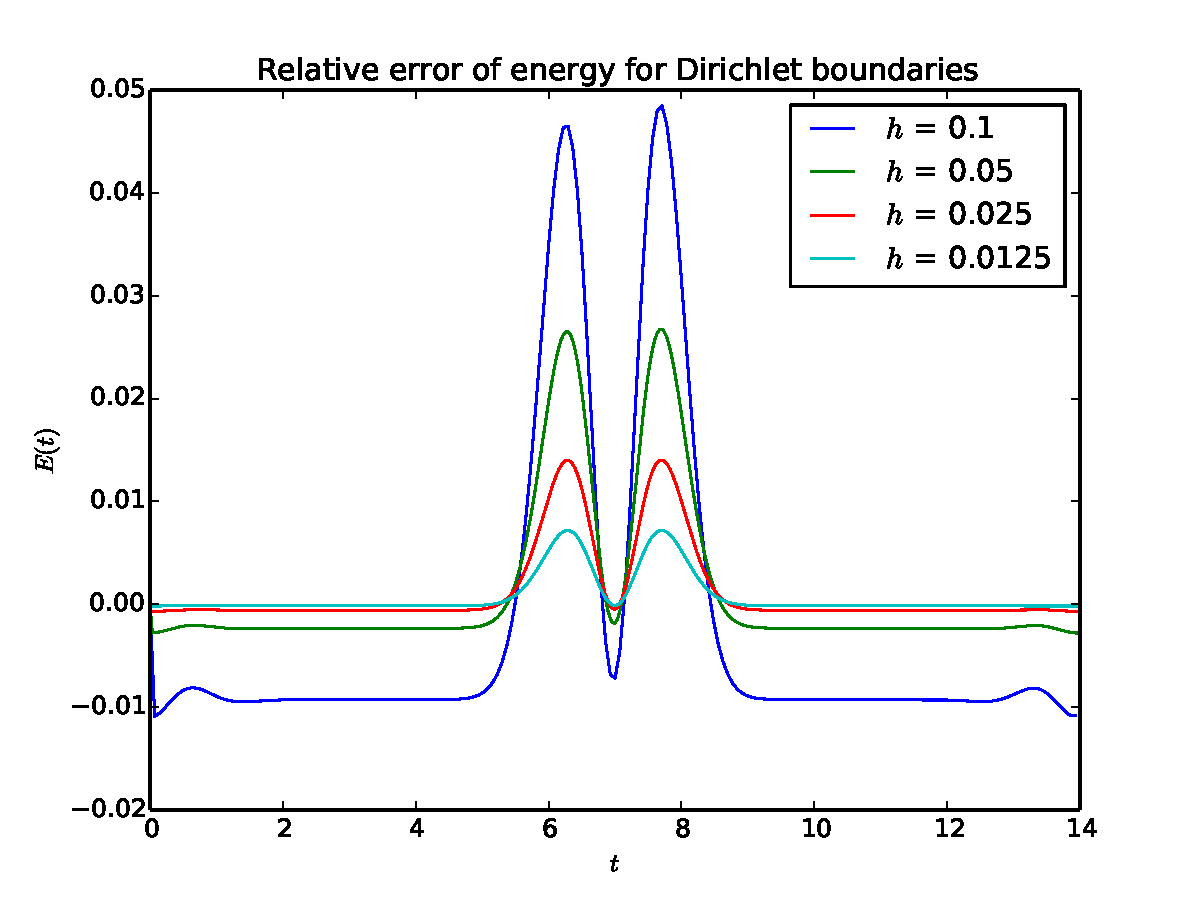
\includegraphics[width=0.5\textwidth]{1/Ed.pdf}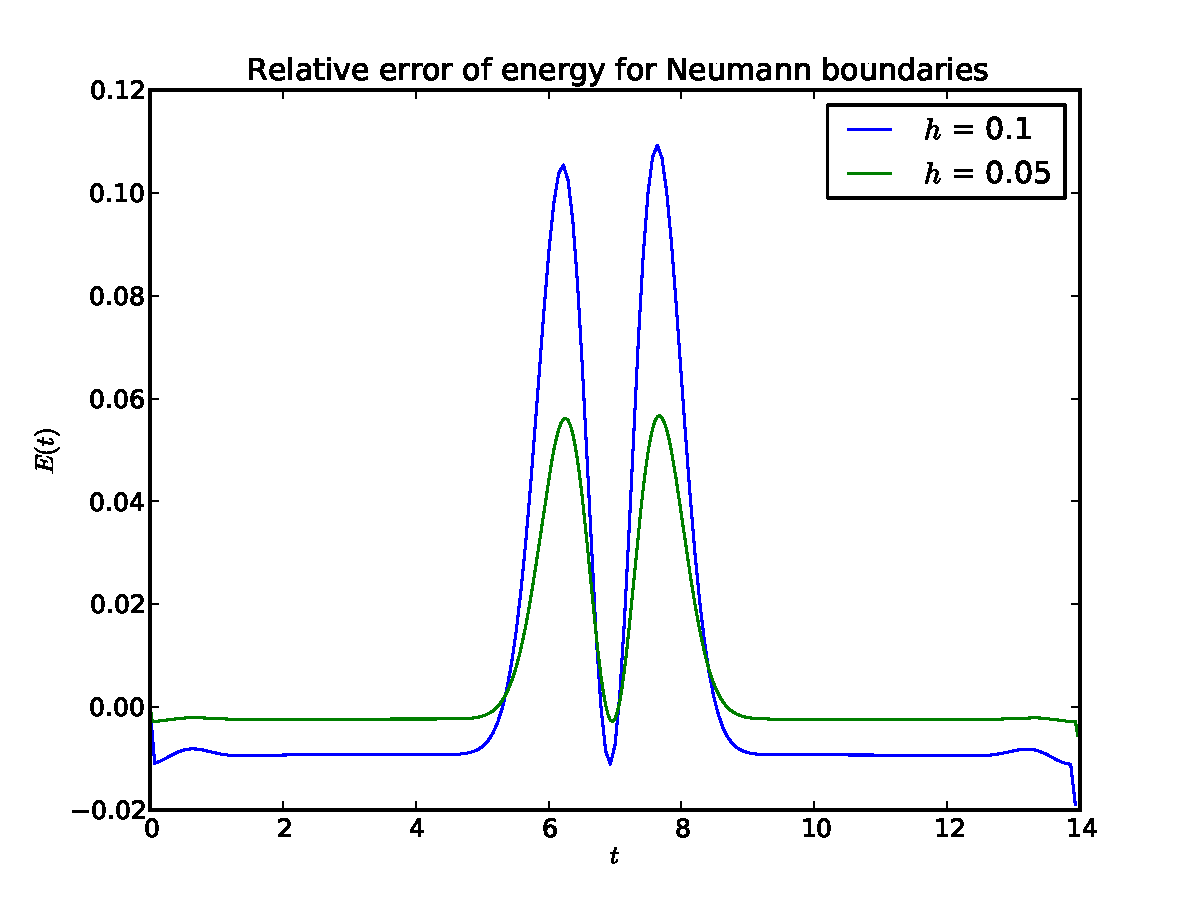
\includegraphics[width=0.5\textwidth]{1/En.pdf}
  \caption{Relative error for Dirichlet(left) and Neumann(Right) boundary conditions.}
  \label{f:relerr}
\end{figure}

For both boundary conditions, we see that the solution is bounded above and below. There
are peaks in the relative error for both cases when the wave is interacting with the boundary
points, and the amplitude of these peaks is slightly over double when Neumann boundary conditions
are used.
The peaks are bounded by a number that appears to scale linearly with $h$, in the sense that halving
$h$ halves the amplitude of these peaks, and so on.

For the majority of the interval $t\in [0,14]$, we see that $f_r(t)$ is bounded below by a
small number, which is $h^{-2}$. Given the $h^{-2}$, $\tau^{-2}$ dependence of
$\mathcal{H}_j^n$ from our integration, this makes sense.
As $t\to14$ however, this bound is broken.


\clearpage
\section*{Question 2}
\subsection*{(1)}
We are now asked to solve the wave equation with $c=1$ and external potential
$V(x) = \frac{1}{\cosh^2(x)}$.
I chose to use central differences -- equation \ref{e:central} -- once again as it
is simple to program and showed no significant shortcomings in the previous
section which cannot be fixed by computational power.
By the same method as for question 1.1, we can use central differences for this
equation. This gives
\begin{equation}
\ujnp = \nu^2 \left[\ujmn + \ujpn \right] - \ujnm + 2(1 - \nu^2)\ujn - \tau^2 V_j \ujn
\label{e:cdp}
\end{equation}
where $V_j$ is the potential corresponding to the $x$-value $j$. The effect of
$V$ can be seen to scale with the time step $\tau$, which is intuitive.

The program was written in Python 3 again, and is in appendix \ref{a:2.1}.
A plot of the waves behaviour is shown in figure \ref{f:cosh}.
After travelling left to the potential barrier, the wave interacts with the barrier,
and some is transmitted, while more is reflected.

\begin{figure}
  \centering
  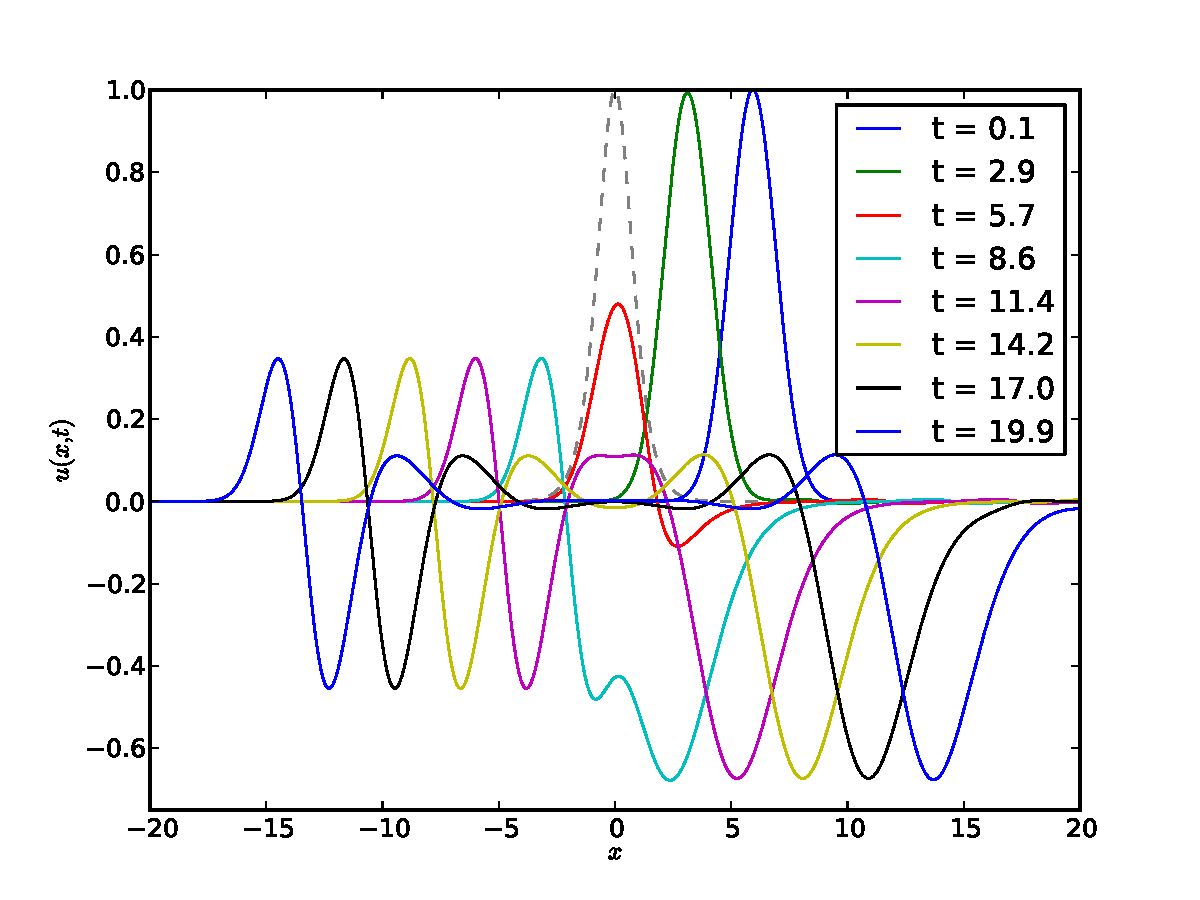
\includegraphics[width=\textwidth]{2/cosh.pdf}
  \caption{The wave at various times, with the potential plotted in the dashed grey line.}
  \label{f:cosh}
\end{figure}



\clearpage
\subsection*{(2)}
To validate our choice of $h$ in the previous section, we perform another study using
the relative error defined in equation \ref{e:err}.
The program which does this operates in the same manner as the previous resolution study,
and is presented in appendix \ref{a:2.2}.

\clearpage
\subsection*{(3)}
We now compute the total energy of the wave as a function of time. As in section
1.5.
We define our Hamiltonian density as in section 1.5, but with
a term for the external potential, giving
\begin{equation}
\mathcal{H}(x,t) = \frac{1}{2}\left(\frac{\partial u}{\partial t}\right)^2
+\frac{1}{2}\left(\frac{\partial u}{\partial x}\right)^2 +\frac{1}{2}V(x)u(x,t)^2,
\label{e:ham}
\end{equation}
making our expression for the numerical $\mathcal{H}$
$$ \mathcal{H}_j^n = \frac{1}{2}\left[\frac{1}{2\tau}\left(\ujnp - \ujnm\right)\right]^2
+ \frac{1}{2}\left[ \frac{1}{2h} \left(\ujpn - \ujmn\right)\right]^2 +
\frac{1}{2}V_j\left(\ujn\right)^2.$$
This is integrated as before, and the results for various values of $h$ are shown in
figure \ref{f:hstudy2}.

\begin{figure}
  \centering
  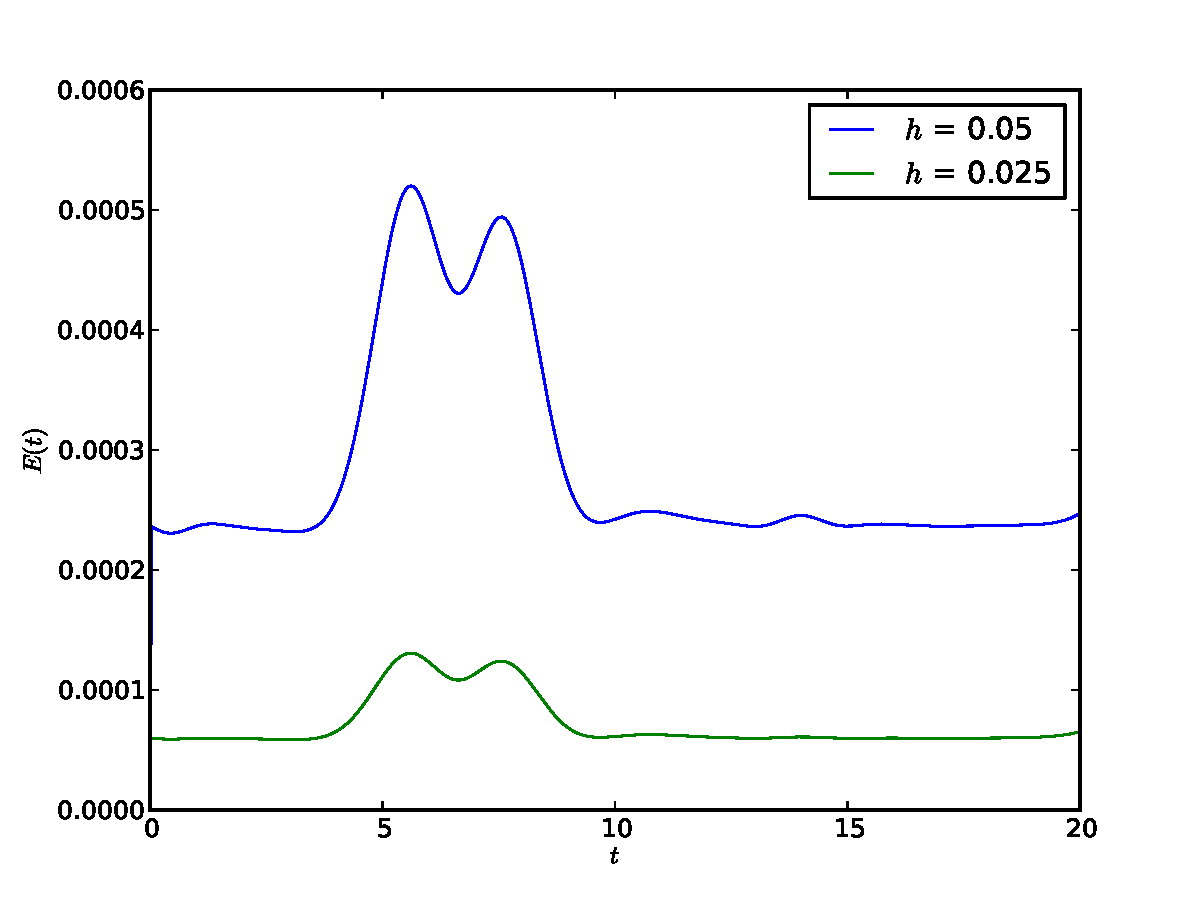
\includegraphics[width=\textwidth]{2/En.pdf}
  \caption{Relative error in energy as a function of time.}
  \label{f:hstudy2}
\end{figure}


\clearpage
\subsection*{(4)}
We are now interested in quantifying how much of the pulse is transmitted through
the potential barrier. We define
\begin{equation}
T_\sigma(t_\text{max}) = \frac{E_<(t_\text{max}) - E(t_\text{max})}{E(t_\text{max})}
\label{e:T}
\end{equation}
as the {\it transmission coefficient} for a given $\sigma$,
where $E_<(t)$ is the energy of the wave left of $x=0$, i.e. the transmitted wave.
This transmission coefficient, $T\in[0,1]$, provides a measure of how much of the pulse
is transmitted for a given $t_\text{max}$ and $\sigma$.
$t_\text{max}$ is chosen so that the wave is sufficiently far from both the potential
barrier and the boundaries to be interacting with neither, and in this case is taken as
$t_\text{max} = 18$.

Figure \ref{f:sigma} shows the dependence of $T$ on $\sigma$. There is a clear
increase in $T$ as $\sigma$ decreases, below $\sigma \sim 2.5$. Above $\sim 2.5$,
the evaluation of $T$ becomes unrepresentative of what is happening, as
the initial Gaussian is spread very wide, with a significant portion already beyond
the barrier, as is seen in figure \ref{f:bigsig}, with $\sigma = 4$.
This can be rectified by changing the value of $\mu$ in the Gaussian to start the
wave further away, but the range of $\sigma$ values presented here is sufficient.

Our initial condition, $\frac{\partial u}{\partial t}(x,0) = \frac{\partial u}{\partial x} (x,0)$,
is largely responsible for the effect of $\sigma$ on $T$. Since we know
$$ u(x,0) = e^{-\frac{(x-\mu)^2}{2\sigma^2}},$$
we can analytically compute $\frac{\partial u}{\partial t}(x,0)$, the initial velocity
of the wave, to be
$$ \frac{\partial u}{\partial t}(x,0) = -\frac{(x-\mu)}{\sigma^2}e^{-\frac{(x-\mu)^2}{2\sigma^2}}. $$
Clearly, the initial velocity of the wave is increased as $\sigma$ is decreased, resulting in
a more energetic wave better able to overcome the barrier.

\begin{figure}
  \centering
  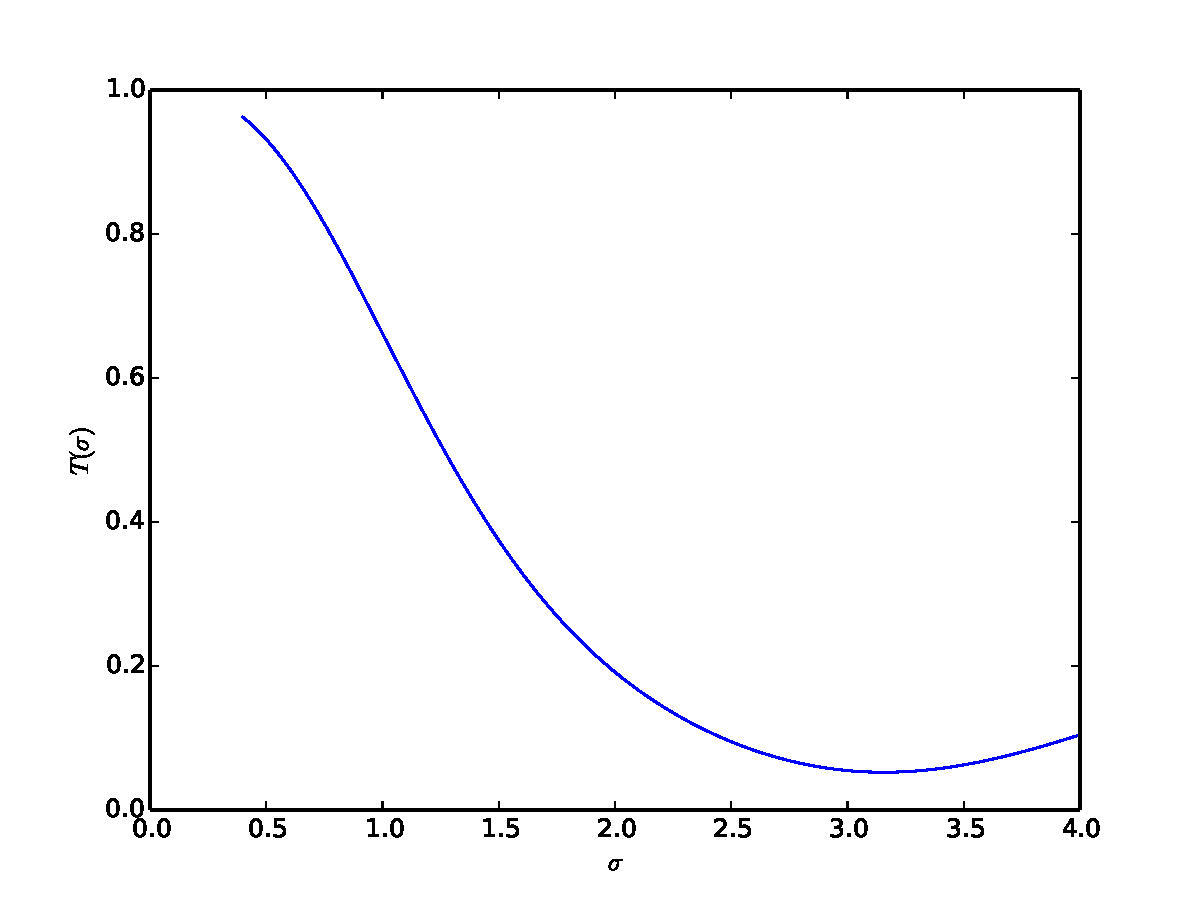
\includegraphics[width=\textwidth]{2/sigma.pdf}
  \caption{Dependence of $T$ on $\sigma$.}
  \label{f:sigma}
\end{figure}

\begin{figure}
  \centering
  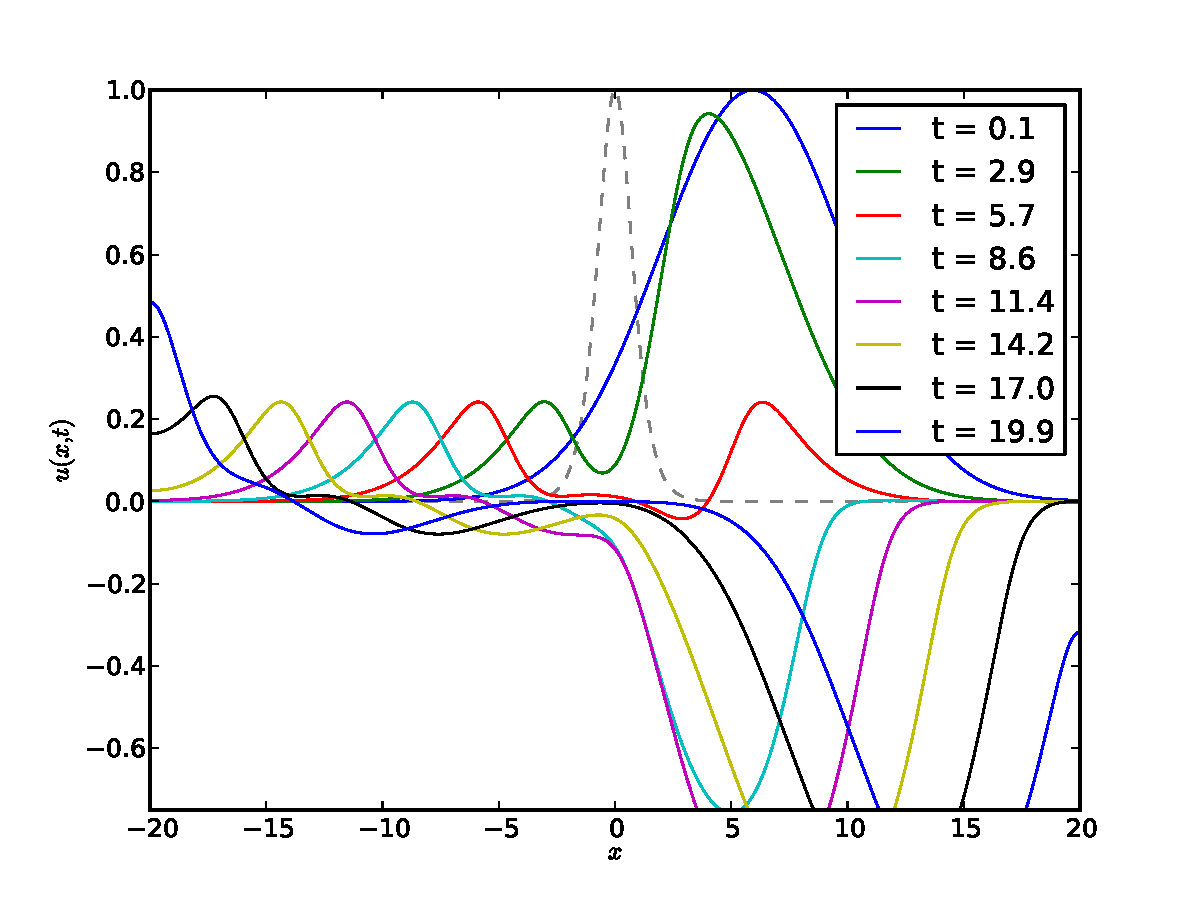
\includegraphics[width=0.7\textwidth]{2/bigsig.pdf}
  \caption{Plot of the system for $\sigma=4$.}
  \label{f:bigsig}
\end{figure}



\newpage
\begin{appendix}
\section{Program for 1.1}
\label{a:1.1}
\lstinputlisting[language=python]{1/dirichlet.py}
\newpage
\section{Program for 1.3}
\label{a:1.3}
\lstinputlisting[language=python]{1/hstudy.py}
\newpage
\section{Program for 1.4}
\label{a:1.4}
\lstinputlisting[language=python]{1/neumann.py}
\newpage
\section{Programs for 1.5}
\label{a:1.5}
{\bf Dirichlet Boundaries}:
\lstinputlisting[language=python]{1/Hd.py}
{\bf Neumann Boundaries}:
\lstinputlisting[language=python]{1/Hn.py}
\newpage
\section{Program for 2.1}
\label{a:2.1}
\lstinputlisting[language=python]{2/potential.py}
\newpage
\section{Program for 2.2}
\label{a:2.2}
\lstinputlisting[language=python]{2/hstudy.py}
\newpage
\section{Program for 2.3}
\label{a:2.3}
\lstinputlisting[language=python]{2/potential.py}
\newpage
\section{Program for 2.4}
\label{a:2.4}
\lstinputlisting[language=python]{2/trans.py}
\end{appendix}



\end{document}
